%Este trabalho está licenciado sob a Licença Atribuição-CompartilhaIgual 4.0 Internacional Creative Commons. Para visualizar uma cópia desta licença, visite http://creativecommons.org/licenses/by-sa/4.0/deed.pt_BR ou mande uma carta para Creative Commons, PO Box 1866, Mountain View, CA 94042, USA.

\chapter{Perceptron}\label{cap_perceptron}
\thispagestyle{fancy}


\section{Unidade de Processamento}

A unidade básica de processamento (neurônio artificial) que exploramos nestas notas é baseado no \emph{perceptron} (consultemos a Fig. \ref{fig:perceptron}). Consiste na composição de uma \emph{função de ativação} $f:\mathbb{R}\to\mathbb{R}$ com a \emph{pré-ativação}
\begin{align}
  z &= \pmb{w}\cdot\pmb{x} + b\\
    &= w_1x_1 + w_2x_2 + \cdots + w_nx_n + b
\end{align}
onde, $\pmb{x}\in\mathbb{R}^{n}$ é o vetor de entrada, $\pmb{w}\in\mathbb{R}^{n}$ é o vetor de pesos e $b\in\mathbb{R}$ é o {\it bias}. Escolhida uma função de ativação, a saída do neurônio é dada por
\begin{align}
  y &:= \mathcal{N}\left(\pmb{x};(\pmb{w},b)\right)\\
    &= f(z) = f(\pmb{w}\cdot\pmb{x} + b)
\end{align}
O treinamento (calibração) consiste em determinar os parâmetros $(\pmb{w}, b)$ de forma que o neurônio forneça as saídas $y$ esperadas com base em algum critério predeterminado.

\begin{figure}[H]
  \centering
  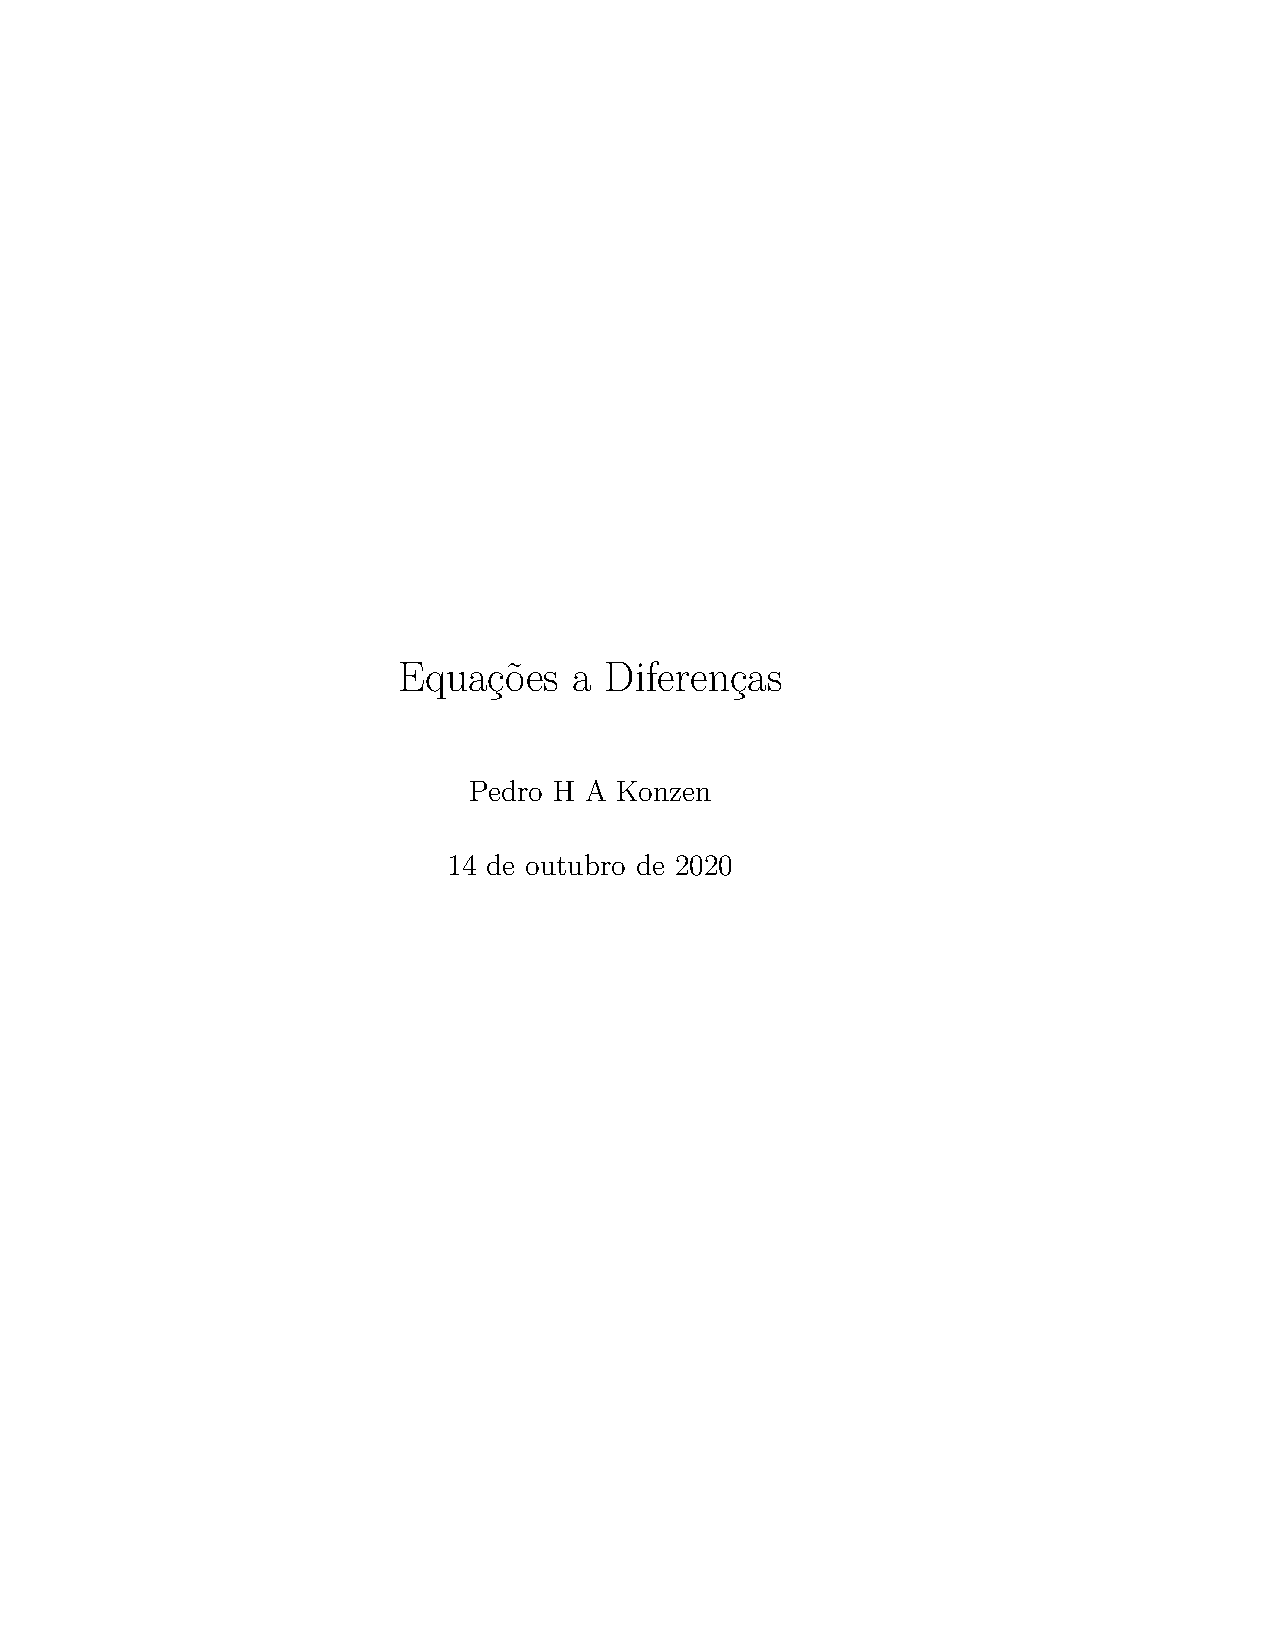
\includegraphics[width=0.7\textwidth]{./cap_perceptron/dados/neuronio/main}
  \caption{Esquema de um perceptron: unidade de processamento.}
  \label{fig:perceptron}
\end{figure}

Uma das vantagens deste modelo de neurônio é sua generalidade, i.e. pode ser aplicado a diferentes problemas. Na sequência, vamos aplicá-lo na resolução de um problema de classificação e noutro de regressão.


\subsection{Um problema de classificação}

Vamos desenvolver um perceptron que faça a operação $\land$ (e-lógico). I.e, receba como entrada dois valores lógicos $A_1$ e $A_2$ (V, verdadeiro ou F, falso) e forneça como saída o valor lógico $R = A_1 \land A_2$. Consultemos a seguinte tabela verdade:

\begin{center}
  \begin{tabular}{cc|c}
    $A_1$ & $A_2$ & R\\\hline
    V & V & V\\
    V & F & F\\
    F & V & F\\
    F & F & F\\\hline
  \end{tabular}
\end{center}


\subsubsection{Modelo}

Nosso modelo de neurônio será um perceptron com duas entradas $\pmb{x}\in \{-1,1\}^2$ e a função sinal
\begin{equation}
  f(z) = \sign(z) = \left\{
    \begin{array}{ll}
      1 &, z>0\\
      0 &, z=0\\
      -1 &, z<0
    \end{array}
\right.
\end{equation}
como função de ativação, i.e.
\begin{equation}
  \mathcal{N}\left(\pmb{x};(\pmb{w},b)\right) = \sign(\pmb{w}\cdot\pmb{x} + b),
\end{equation}
onde $\pmb{w}\in\mathbb{R}^2$ e $b\in\mathbb{R}$ são parâmetros a determinar.


\subsubsection{Pré-processamento}

Uma vez que nosso modelo recebe valores $\pmb{x}\in \{-1,1\}^2$ e retorna $y\in\{-1,1\}$, precisamos (pre)processar os dados do problema de forma a utilizá-lo. Uma forma, é assumir que todo valor negativo está associado ao valor lógico $F$ (falso) e positivo ao valor lógico $V$ (verdadeiro). Desta forma, os dados podem ser interpretados como na seguinte tabela

\begin{center}
  \begin{tabular}{rr|c}
    $x_1$ & $x_2$ & $y$\\\hline
    1 & 1 & 1\\
    1 & -1 & -1\\
    -1 & 1 & -1\\
    -1 & -1 & -1\\\hline
  \end{tabular}
\end{center}
    
    
\subsubsection{Treinamento}

Agora, nos falta treinar nosso neurônio para fornecer o valor de $y$ esperado para cada dada uma entrada $\pmb{x}$. Isso consiste em um método para escolhermos os parâmetros $(\pmb{w},b)$ que sejam adequados para esta tarefa. Vamos explorar mais sobre isso na sequência do texto e, aqui, apenas escolhemos
\begin{gather}
  \pmb{w} = (1, 1)\\
  b = -1
\end{gather}
Com isso, nosso perceptron é
\begin{equation}
  \mathcal{N}(\pmb{x}) = \sign(x_1 + x_2 - 1)
\end{equation}
Verifique que ele satisfaz a tabela verdade acima!


\subsubsection{Implementação}

\ifispython
Podemos implementar nosso perceptron usando {\python}+{\pytorch} como segue

\lstinputlisting{./cap_perceptron/dados/py_e/main.py}

Verifique! Aqui e nas seguintes implementações, utilizamos vários métodos para a manipulação de tensores \lstinline+torch.Tensor+). Consulte \href{https://pytorch.org/docs/stable/torch.html}{PyTorch Docs: torch} para mais informações sobre estes e muitos outros métodos disponíveis.
\fi

\subsubsection{Interpretação geométrica}

Empregamos o seguinte modelo de neurônio
\begin{equation}
  \mathcal{N}\left(\pmb{x};(\pmb{w},b)\right) = \sign(w_1x_1 + w_2x_2 + b)
\end{equation}
Observamos que
\begin{equation}
  w_1x_1 + w_2x_2 + b = 0
\end{equation}
corresponde à equação geral de uma reta no plano $\tau: x_1\times x_2$. Esta reta divide o plano em dois semiplanos
\begin{align}
  \tau^+ = \{\pmb{x}\in\mathbb{R}^2: w_1x_1 + w_2x_2 + b > 0\}\\
  \tau^- = \{\pmb{x}\in\mathbb{R}^2: w_1x_1 + w_2x_2 + b < 0\}
\end{align}
O primeiro está na direção do vetor normal a reta $\pmb{n} = (w_1, w_2)$ e o segundo na sua direção oposta. Com isso, o problema de treinar nosso neurônio para nosso problema de classificação consiste em encontrar a reta
\begin{equation}
  w_1x_1 + w_2x_2 + b = 0
\end{equation}
de forma que o ponto $(1,1)$ esteja no semiplano positivo $\tau^+$ e os demais pontos no semiplano negativo $\tau^-$. Consulte a Figura \ref{fig:}.

\begin{figure}[H]
  \centering
  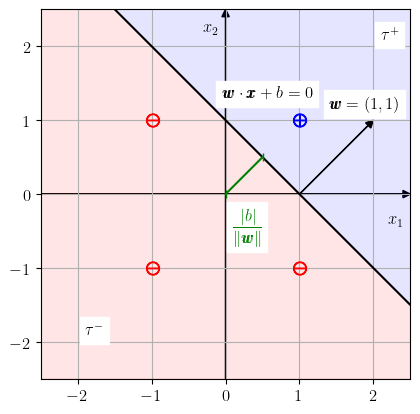
\includegraphics[width=0.7\textwidth]{./cap_perceptron/dados/fig_class_e/main}
  \caption{Interpretação geométrica do perceptron aplicado ao problema de classificação ralacionado à operação lógica $\land$ (e-lógico).}
  \label{fig:}
\end{figure}

\subsubsection{Algoritmo de treinamento: perceptron}

O algoritmo de treinamento perceptron permite calibrar os pesos de um neurônio para fazer a classificação de dados linearmente separáveis. Trata-se de um algoritmo para o \emph{treinamento supervisionado} de um neurônio, i.e. a calibração dos pesos é feita com base em um dado \emph{conjunto de amostras de treinamento}.

Seja dado um \emph{conjunto de treinamento} $\{\pmb{x}^{(s)},y^{(s)}\}_{s=1}^{n_s}$, onde $n_s$ é o número de amostras. O algoritmo consiste no seguinte:
\begin{enumerate}
\item Sete $\pmb{w} = \pmb{0}$, $b=0$.
\item Para $e = 1,\dotsc, n_e$:
  \begin{enumerate}
  \item Para $s = 1,\dotsc, n_s$:
    \begin{enumerate}
    \item Se $y^{(s)}\mathcal{N}\left(\pmb{x}^{(s)}\right) \leq 0$:
      \begin{enumerate}
      \item $\pmb{w} = \pmb{w}+y^{(s)}\pmb{x}^{(s)}$
      \item $b = b + y^{(s)}$
      \end{enumerate}
    \end{enumerate}
  \end{enumerate}
\end{enumerate}
onde, $n_e$ é um dado número de épocas\footnote{Número de vezes que as amostrar serão percorridas para realizar a correção dos pesos.}.

\ifispython
Podemos implementar nosso algoritmo perceptron usando {\python}+{\pytorch} como segue

\lstinputlisting{./cap_perceptron/dados/py_percep_e/main.py}

Verifique!
\fi


\subsection{Problema de regressão}

\emconstrucao

